
%\documentclass[pre,preprint,showpacs,nofootinbib]{revtex4}
\documentclass[pre,preprint]{revtex4}
%\documentclass[article]{revtex4}
\usepackage{graphicx}
\usepackage{epsfig}
%\usepackage{dcolumn}
\usepackage{amssymb,amsmath}
\usepackage{bm}
\usepackage{pdfsync}

\newcommand{\lb}{{\langle}}
\newcommand{\rb}{{\rangle}}

\begin{document}

\title{The Diameter and Chemical Distance of Random Clusters}

\author{Don Blair}
\author{Jon Machta}

\affiliation{Department of Physics, University of Massachusetts, Amherst, MA 01003.}
\date{\today}


 \begin{abstract}
  A relatively unexplored geometric property of Potts models clusters is their ``diameter'', $w$ -- the longest shortest path between any two points on the cluster. We report the results of numerical simulations for the fractal dimension of the diameter, $w_{min}$ and the fractal dimension of the chemical distance, $d_{min}$, for 2D critical Potts clusters with $q=1,2,3,4,5$ in 2D, and $q=2$ in 3D and 4D. We find that $D_{min} = d_{min}$ within error.
 \end{abstract}

\maketitle 
\subsection{Introduction}
The  $q$-state Potts Model \cite{Po52} contains the Ising Model and the Percolation Model as special cases (($q \to 2$ and $q \to 1$, respectively), and can be generalized to the random-cluster model for all $q \ge 0$ \cite{FoKa}. Though relatively simple to formulate, the Potts Model model exhibits rich phase behavior, and its study has yielded many significant insights into critical phenomena.  While the several critical exponents of the two-dimensional  $q$-state Potts model have been solved for exactly, some remain elusive; one such critical exponent -- describing an important geometric property of Potts clusters, with no apparent thermodynamic analog -- is the fractal dimension $d_{min}$ of the ``chemical'' or ``shortest'' path, $l$, on Potts clusters.  Much work has already been done to determine $d_{min}$ numerically \cite{Gr83, HrSt88} for the $q=1$, 2D Potts Model (percolation), and some promising attempts have been made at exact solutions using results from conformal field theory \cite{Zi99}, [Sokal].  Currently, no relationship between the $d_{min}$ and other scaling exponents has been conclusively established [REFS].

In this paper, we extend previous studies of $d_{min}$ to include the $q=2,3,4$ in 2D, and $q=2$ (Ising) in 3D and 4D. For the systems, we also study the scaling of a new geometric property of critical Potts clusters, their ``diameter'', $w$ -- defined as the longest short path path on a cluster -- and compare this scaling exponent, $w_{min}$ with $d_{min}$.

Since $w$ and $l$ are not conventional thermodynamics quantities that can be computed using the renormalization group, it is not clear whether the mean field predictions hold.  We compare our results to the expectations of mean field theory below.

% Since diam is not a conventional thermodynamic quantity that can be computed
% using the renormalization group  it is not clear whether the upper critical
% dimension is a meaningful concept; we thereforeor the above values of  d_min are correct
% above the upper critical dimension.

%Brief review of the Potts Model %

The $q$-state Potts model consists of a lattice of Potts spin variables $\sigma_i$, each of which can have integer values $\sigma_i = 1 \dots q$.  Any two neighboring spins $\sigma_i$ and $\sigma_j$ contribute an amount $-K$ to the Hamiltonian if they have the same value, or zero otherwise; the Hamiltonian can thus be written as:

\begin{equation}
\mathcal{H} = -K \sum_{\lb i,j \rb} \delta_{\sigma_i, \sigma_j},
\end{equation}     

with $K$ a dimensionless coupling constant.  

Our study focuses on the 2D Potts Model on a square lattice.  Clusters in this model are defined by drawing bonds between nearest neighbor sites (where the four nearest neighbors of a site are those sites ``above'', ``below'', ``to the left'', and ``to the right'' of the site) with the same value of the Potts spin variable $\sigma$.  An example such a cluster is shown in Figure \ref{fig: grid}.

In order to define most readily the chemical path and the diameter on Potts Model clusters, let us consider the special case of the Percolation Model (equivalent to the $q \to 1$ case of the Potts model) on the square lattice.  In the Percolation Model, each edge or bond on the lattice is either ``occupied" (with probability $p$) or ``empty'' (with probability $1-p$). For $0 < p < 1$, finite-sized clusters of sites connected by bonds will form; at some critical value $p_c = 1/2$ there first appears, on average, a cluster that spans the lattice \cite{Stau96} (connecting, e.g., the top row of the square lattice to the bottom). 

The chemical path is illustrated for a particular realization of a $9$-by-$9$ Percolation Model lattice.  Let us choose any two sites $A_1$ and $A_2$ on a cluster in the lattice, separated by a Euclidean distance $r$.  The shortest path $l$ along cluster bonds that connect the sites $A_1$ and $A_2$ is the ``chemical path'' \cite{HrHoSt84} between the two sites.  The average length of the chemical path for clusters at criticality behaves as $\bar{l} \propto r^{d_{min}}$, where $d_{min}$ is the scaling dimension of $\bar{l}$. These quantities are illustrated for an example percolation cluster in a $9$-by-$9$ square grid in Figure \ref{fig: griddotschem}.

The diameter $D$ may then be defined as follows:  first, form the set $s$ of all possible shortest paths on the cluster by determining the shortest paths $l$ between all possible pairs of sites $(A_i, A_j)$ on the cluster. The largest path in $S$ is the ``diameter'', $w$, of the cluster.  In other words: $w$ is the ``longest shortest path'' on the cluster.  The diameter is illustrated in Figure \ref{fig: griddotsdiam}.

We expect that $\bar{D}$ also exhibits scaling behavior at criticality: $\bar{w} \propto r^{w_{min}}$.

We are performing Monte Carlo simulations of critical $q$-state Potts model clusters using the Swendsen-Wang algorithm (SW) \cite{SwWa86, NeBa99}.  The SW algorithm, which is itself based on the work of Fortuin and Kasteleyn \cite{FoKa}, works by first introducing bonds between neighboring spins, with probability 

\begin{equation}
p(\sigma_i,\sigma_j) = \delta_{\sigma_i, \sigma_j} (1-e^{-K}),
\end{equation}  

thus creating clusters of bonded spins.   All clusters thus formed are then, with probability 1/2, ``flipped'' by choosing a random spin value (a new Potts state, different from the current state of the cluster's spins) from the $q-1$ possible values, and assigning this value to all sites in the cluster.  Such ``cluster-flipping'' algorithms dramatically reduce critical slowing down in computer simulations of spin models, as compared with algorithms that flip each spin individually \cite{NeBa99} (e.g. the Metropolis algorithm \cite{Met}). 

Identifying the diameter $w$ of a cluster is a computationally expensive, order $n^2$ operation, as it requires. identifying all shortest paths among all pairs on the cluster.  We therefore restricte our study of the $w$ and $l$ to $L \le 128$. 

% , of a Potts cluster would seem require finding the shortest paths between all pairs of sites in the cluster.  This ``all-pairs shortest paths'' problem has been studied extensively in computer science\cite{Fred87}.  We believe we have developed a diameter-finding algorithm that saves significant time as compared to computing all-pairs shortest paths in the cluster, by exploiting the fact that our clusters are embedded in 2D square lattices.  We are as yet unsure whether there exists a faster algorithm in the literature that accomplishes the same task and is as straightforward to implement.  

\subsection{Methods}

We used the Swendsen Wang algorithm to simulate the Potts Model for $q=1,2,3,4$ on 2D square lattices of various sizes $L$, and for $q=2$ in 3D and 4D cubic and hypercubic lattices.  In 2D, $L$ ranged from 16 to 128; in 3D, from 20 to 128; and in 4D, from 12 to 64. For 2D, $q=1$, the chemical distance $l$ and the diameter $D$ were measured after every Monte Carlo sweep, for a total of $N=10^5$ measurements. For 2D $q>1$, the systems were allowed to equilibrate: 100 initial sweeps of the lattice were discarded at the beginning of each simulation, and an additional $10*\tau_{exp}(m)$ sweeps were discarded after data was collected, where $\tau_{exp}$ was the measured exponential correlation \cite{Ah91} time of the mass of the largest cluster in each lattice. In order to further reduce correlations in the data for $q>1$ in 2D, an interval of 10 sweeps separated each measurement during the simulation; this interval was always greater than $2\tau_{int}(y)$, where $\tau_{int}(y)$ was the measured value of the integrated correlation time of $y$ ( $y=l$, or $D$). The total number of measurements made in this manner for 2D, $q>1$ was $N=10^5$; for the 2D, $q=4$, $L=128$ lattice, this amounted to a simulation time of approximately $3.1 \times 10^5 \tau_{int}(D)$.  In 3D and 4D, measurements were made every Monte Carlo sweep for a total of $N=10^5$ measurements.  For all lattices in 2D, 3D, and 4D with $q>1$, the estimated standard deviation in the averaged values of $l$ and $D$ was considered to be $\sigma_{corr} = \sqrt{ \frac{2 \tau_{int}(y)}{N} (\lb y^2 \rb - \lb y \rb^2)}$.  For $q=1$, the standard deviation was calculated as $\sigma_{uncorr} = \sqrt{ \frac{1}{N-1} (\lb y^2 \rb - \lb y \rb^2)}$.

In order to determine the value of $B$ in the scaling Ansatz $y=AL^{B}$ (where $y$ is equal to $l$ or $D$, and $B$ is equal to, respectively, $d_{min}$ or $D_{min}$), we performed a weighted least-squares fit using the Levenberg-Marquardt [REF] that minimized $((y-data)/\sigma))^2$, where $\sigma$ was defined as above. The resultant fits are displayed in Figures \ref{fig:a} through \ref{fig:b} below.  A summary of the fit results for the scaling exponents $B=l_{min}$ and $D_{min}$ is reported in Tables \ref{tab:D2vals} and \ref{tab:D3and4vals} as $B \pm \sqrt{\nu_B}$, where $\nu_{B}$ is the diagonal element of the covariance matrix corresponding to parameter $B$.

To account for corrections to scaling, we performed fits on subsets of the data with a variable lower $L$ cutoff of $L_{min}$, and chose to report the value of $B$ that resulted from including the smallest $L_{min}$ where the goodness of fit $Q>.2$; $Q$ is the incomplete gamma function $Q(p/2,\chi^2/2)$, defined [REF Numerical Recipes (6.2.3)] as $\frac{1}{\Gamma(p)}\int_x^{\infty}e^{-t}t^{p-1}dt$, with $p$ being the number of degrees of freedom in the fit. 

For $q=4$ in 2D, we also attempted a fit of the form $y=AL\log{L}(1+B/L)$, which yielded $Q$ values much lower than those resulting from the corresponding $y=AL^{B}$ fits.

\subsection{Results}

\subsection{Discussion}

\subsubsection {Expectations from mean field theory}

From Nachmias and Peres, for the percolation problem on the complete graph
at criticality one has:

\begin{itemize}
\item Complete graph at criticality: $w(n) ~ n^{1/3}$

\item Upper critical dimension (dim above which mean field exponents hold) for $q=1$ (percolation) is 6 [REFS];

\item Therefore, $L^6=n$ is mapping from $n$ to a linear dimension.  

\item Therefore, $w(L) ~ L^2$; so $d_{min}$ should approach $2$ as $dim$ approaches 6.

\item For $q=2$ (Ising) model there exist two random graphs (+ spins and - spins) [REFS], and at
criticality $w(n)~n^{1/3}$.  The upper critical dimension is for $q=2$ is 4 [REFS], so $L^4=n$, and $d_{min}$ should therefore approach 4/3 as $dim$ approaches 6. 
\end{itemize}

% Since diam is not a conventional thermodynamic quantity that can be computed
% using the renormalization group  it is not clear whether the upper critical
% dimensions is a meaningful concept or the above values of d_min are correct
% above the upper critical dimension.


\subsubsection {Comparison of $d_{min}$ and $w_{min}$}

\subsubsection{ Mention of Sokal's results}


%\section{Tables}

\begin{center}
\begin {table}[ht]
\addtolength{\tabcolsep}{5pt}
%\caption{Scaling exponents $d_{min}$ and $D_{min}$ for $dim=2$, $q=1,2,3,4$}
\begin{tabular}{|c| c |c|c|c|c|}
\hline
 dim  &  $q$  &  $L$                   &  $L_{min}$  &   $d_{min}$  &   $D_{min}$  \\
\hline
   2  &  1  &  16,32,48,64,96,128  &       48  &  1.131(1)  &  1.138(1)  \\
   2  &  2  &  16,32,48,64,96,128  &       48  &  1.096(1)  &  1.102(1)  \\
   2  &  3  &  16,32,48,64,96,128  &       48  &  1.065(3)  &  1.071(1)  \\
   2  &  4  &  16,32,48,64,96,128  &       48  &  1.033(3)  &  1.039(1)  \\
\hline
\end{tabular}
\caption{Scaling exponents $d_{min}$ and $D_{min}$ for $dim=2$, $q=1,2,3,4$}
\label{tab:D2vals}
\end{table}
%\caption{Scaling exponents $d_{min}$ and $D_{min}$ for $dim=2$, $q=1,2,3,4$}
\end{center}


%\begin{tabular}{rrlrrl}
\begin{center}
\begin {table}[ht]
\addtolength{\tabcolsep}{5pt}
%\caption{Scaling exponents $d_{min}$ and $D_{min}$ for $dim=3,4$, $q=2$}
\begin{tabular}{|c| c |c|c|c|c|}
\hline
dim  &  $q$  &  $L$                   &  $L_{min}$  &   $d_{min}$  &   $D_{min}$  \\
\hline
   3  &  2  &  20,36,48,64,128  &       36  &  1.267(5)  &  na       \\
   4  &  2  &  12,24,36,48,64   &       24  &  1.485(7)  &  na       \\
\hline
\end{tabular}
\caption{Scaling exponents $d_{min}$ and $D_{min}$ for $dim=3,4$, $q=2$}
\label{tab:D3and4vals}
\end{table}
\end{center}

%\section{Figures}


% Figures for D=2:

% q=1, d_min

\begin{figure}[htp]
\centering
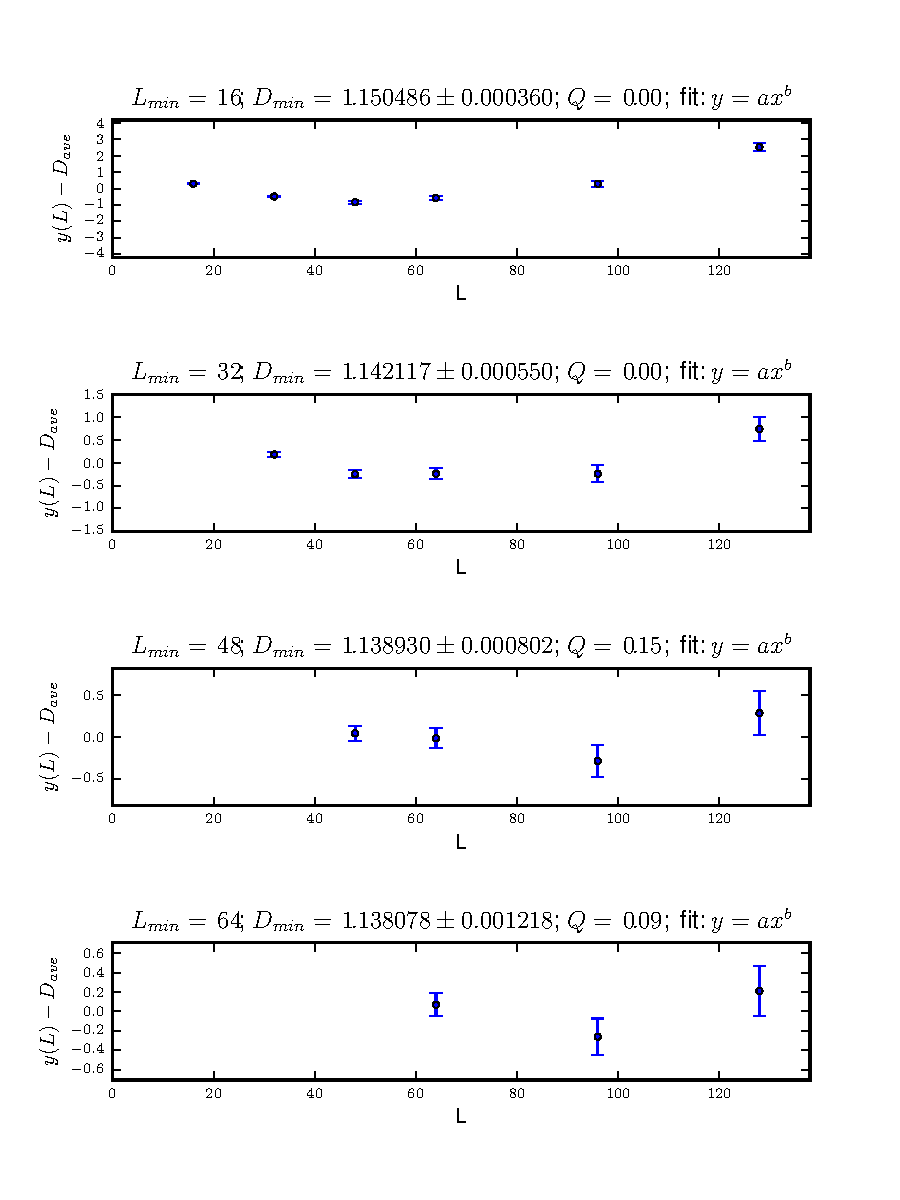
\includegraphics[width=.85\textwidth]{figures/d_min_D2q1_46_fig}
\caption{The difference between the fit, $y(L)=cL^{d_{min}}$, and the average chemical distance $\lb l \rb$ for dim=2, q=1.}\label{fig:a}
\end{figure}

%q=1, D

\begin{figure}[htp]
\centering
\includegraphics[width=.85\textwidth]{figures/D_min_D2q1_46_fig}
\caption{The difference between the fit, $y(L)=cL^{D_{min}}$, and the average diameter $\lb D \rb$ for dim=2, q=1.}\label{fig:2}
\end{figure}


%q=2, d

\begin{figure}[htp]
\centering
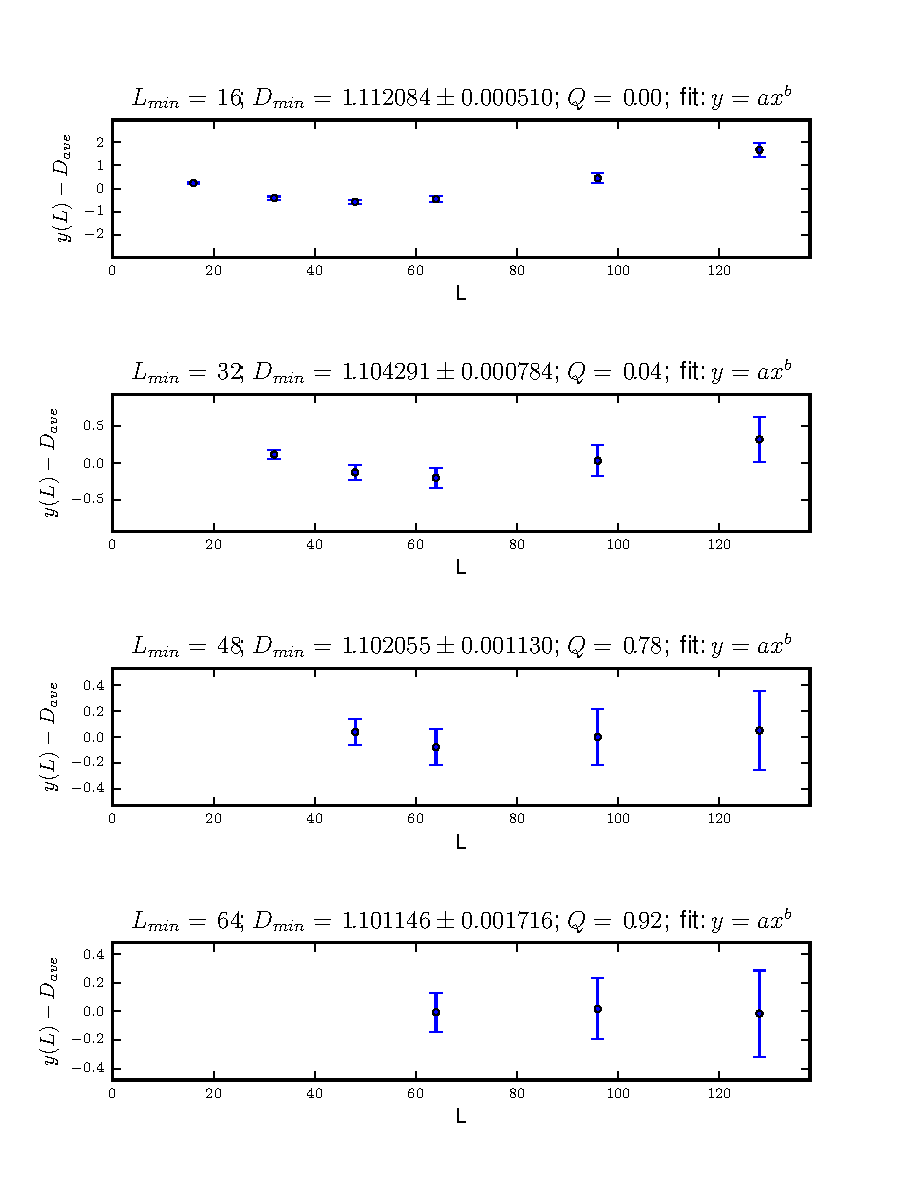
\includegraphics[width=.85\textwidth]{figures/d_min_D2q2_46_fig}
\caption{The difference between the fit, $y(L)=cL^{d_{min}}$, and the average chemical distance $\lb l \rb$ for dim=2, q=2.}\label{fig:3}
\end{figure}

%q=2, D

\begin{figure}[htp]
\centering
\includegraphics[width=.85\textwidth]{figures/D_min_D2q2_46_fig}
\caption{The difference between the fit, $y(L)=cL^{D_{min}}$, and the average diameter $\lb D \rb$ for dim=2, q=2.}\label{fig:4}
\end{figure}

%q=3, d

\begin{figure}[htp]
\centering
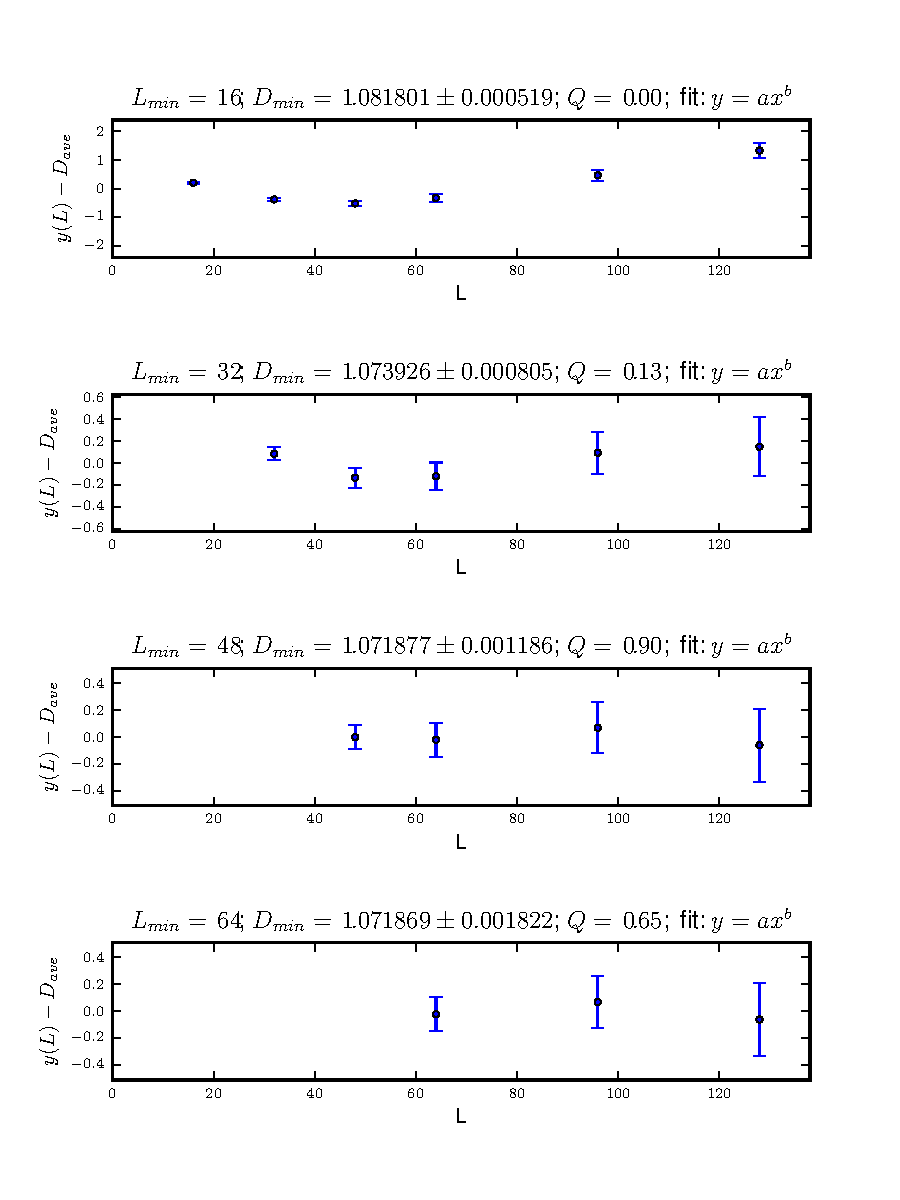
\includegraphics[width=.85\textwidth]{figures/d_min_D2q3_46_fig}
\caption{The difference between the fit, $y(L)=cL^{d_{min}}$, and the average chemical distance $\lb l \rb$ for dim=2, q=3.}\label{fig:4}
\end{figure}

%q=3, D

\begin{figure}[htp]
\centering
\includegraphics[width=.85\textwidth]{figures/D_min_D2q3_46_fig}
\caption{The difference between the fit, $y(L)=cL^{D_{min}}$, and the average diameter $\lb D \rb$ for dim=2, q=3.}\label{fig:4}
\end{figure}

%q=4, d

\begin{figure}[htp]
\centering
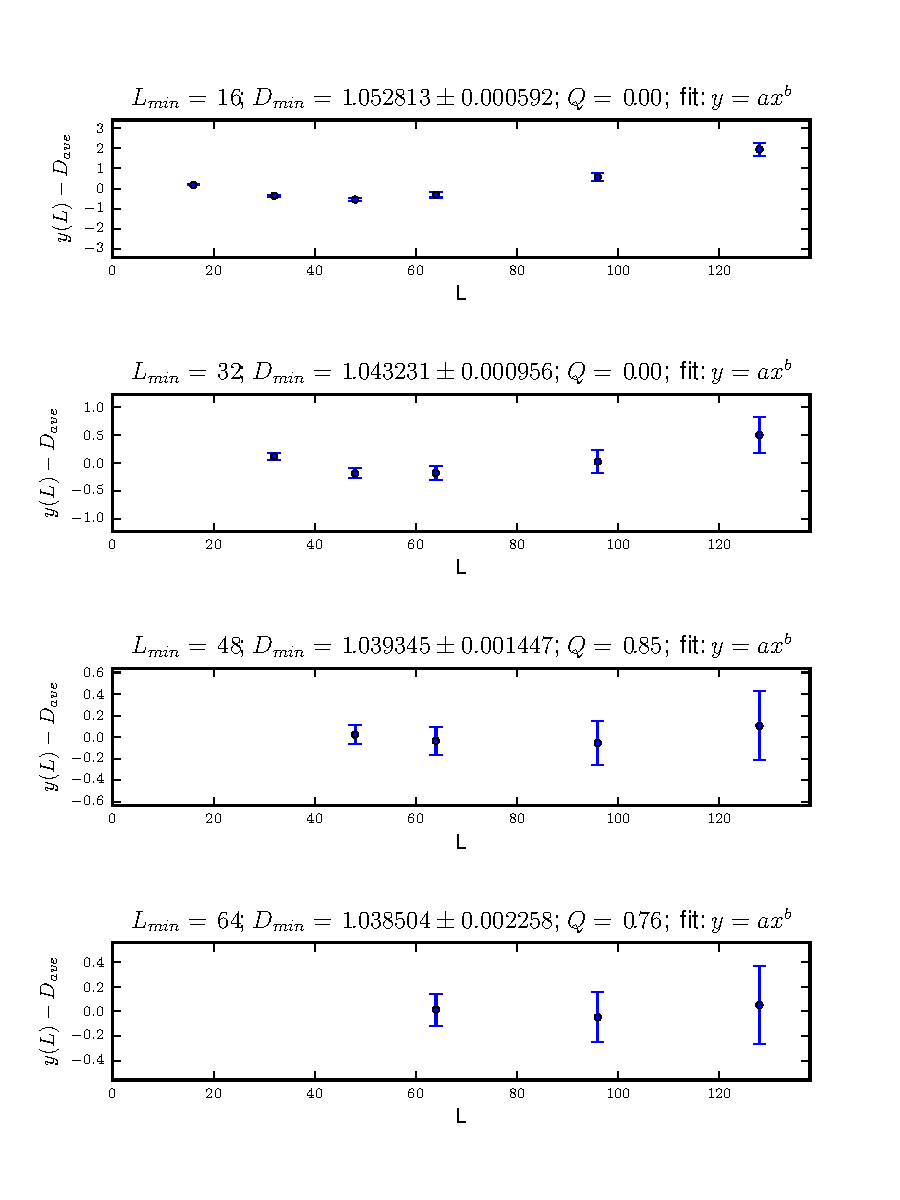
\includegraphics[width=.85\textwidth]{figures/d_min_D2q4_46_fig}
\caption{The difference between the fit, $y(L)=cL^{d_{min}}$, and the average chemical distance $\lb l \rb$ for dim=2, $q$=4.}\label{fig:4}
\end{figure}

%q=4, D

\begin{figure}[htp]
\centering
\includegraphics[width=.85\textwidth]{figures/D_min_D2q4_46_fig}
\caption{The difference between the fit, $y(L)=cL^{D_{min}}$, and the average diameter $\lb D \rb$ for dim=2, $q$=4.}\label{fig:4}
\end{figure}

%q=4, d, log fit

\begin{figure}[htp]
\centering
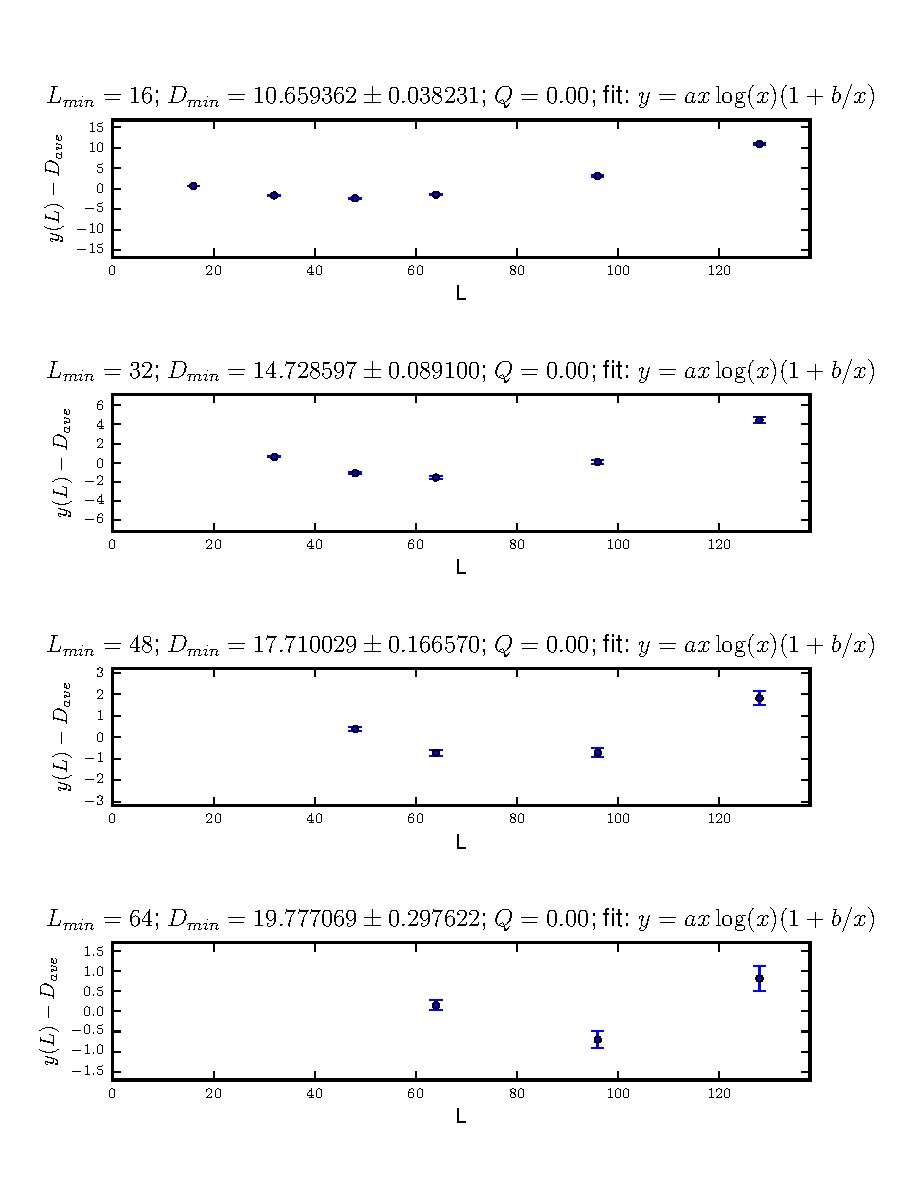
\includegraphics[width=.85\textwidth]{figures/d_min_D2q4_46_log_fig}
\caption{The difference between the fit, $y=AL\log{L}(1+B/L)$ and the average chemical distance, $\lb l \rb$ for dim=2, $q$=4.}\label{fig:4}
\end{figure}

%q=4, D, log fit

\begin{figure}[htp]
\centering
\includegraphics[width=.9\textwidth]{figures/D_min_D2q4_46_log_fig}
\caption{The difference between the fit, $y=AL\log{L}(1+B/L)$ and the average diameter, $\lb D \rb$ for dim=2, $q$=4.}\label{fig:4}
\end{figure}


%D=3, q=2

\begin{figure}[htp]
\centering
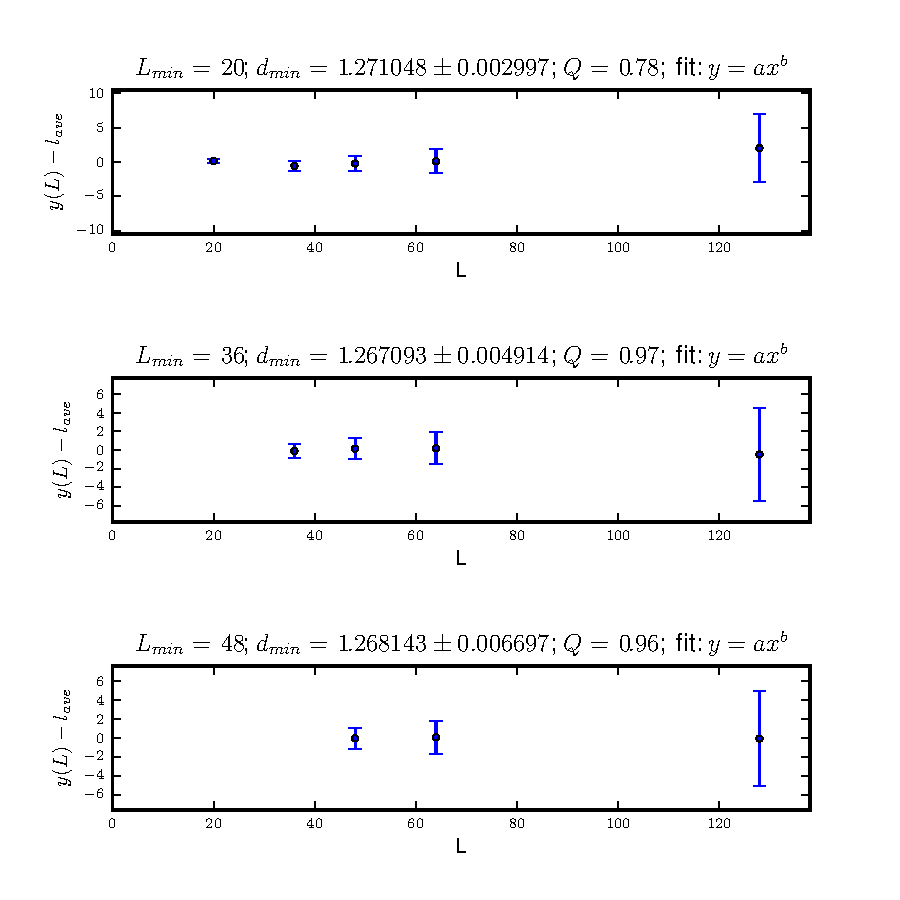
\includegraphics[width=.9\textwidth]{figures/d_min_D3q2_46_fig}
\caption{The difference between the fit, $y(L)=cL^{d_{min}}$, and the average diameter $\lb l \rb$ for dim=3, $q$=2.}\label{fig:4}
\end{figure}

%D=4, q=2

\begin{figure}[htp]
\centering
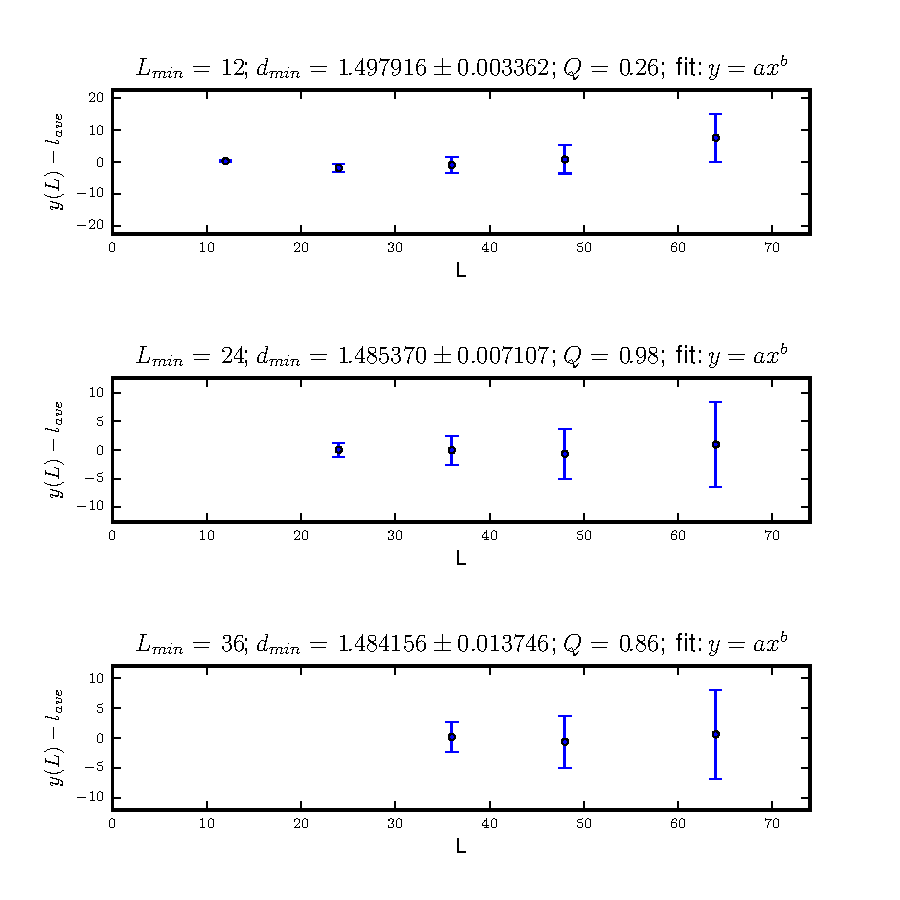
\includegraphics[width=.9\textwidth]{figures/d_min_D4q2_46_fig}
\caption{The difference between the fit, $y(L)=cL^{d_{min}}$, and the average diameter $\lb l \rb$ for dim=4, $q$=2.}\label{fig:b}
\end{figure}

\begin{figure}[htp]
\centering
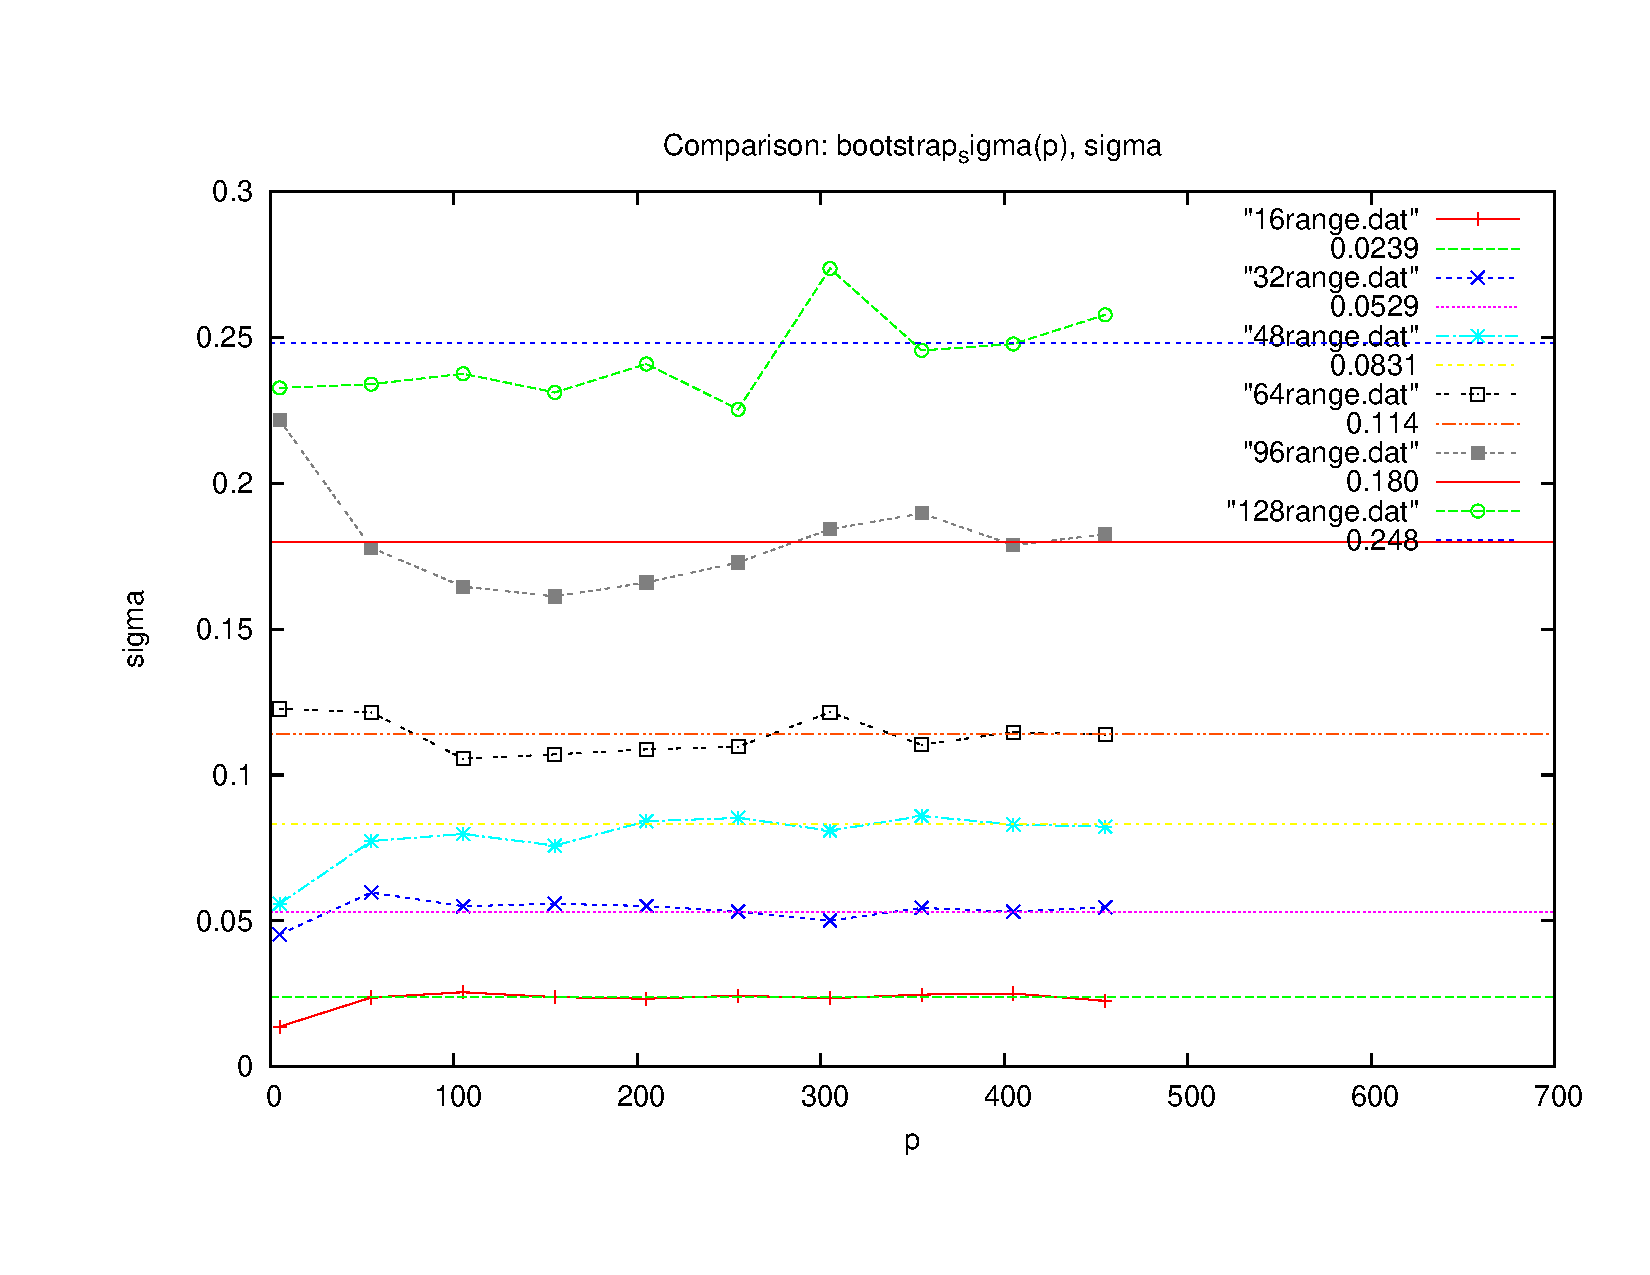
\includegraphics[width=.9\textwidth]{figures/boot}
\caption{$D=2, q=1, d_{min}$: comparison between $\sigma$ calculated as per the above description ``Methods'', and the bootstrap method with $p$ iterations.}\label{fig:b}
\end{figure}

\begin{figure}[htp]
\centering
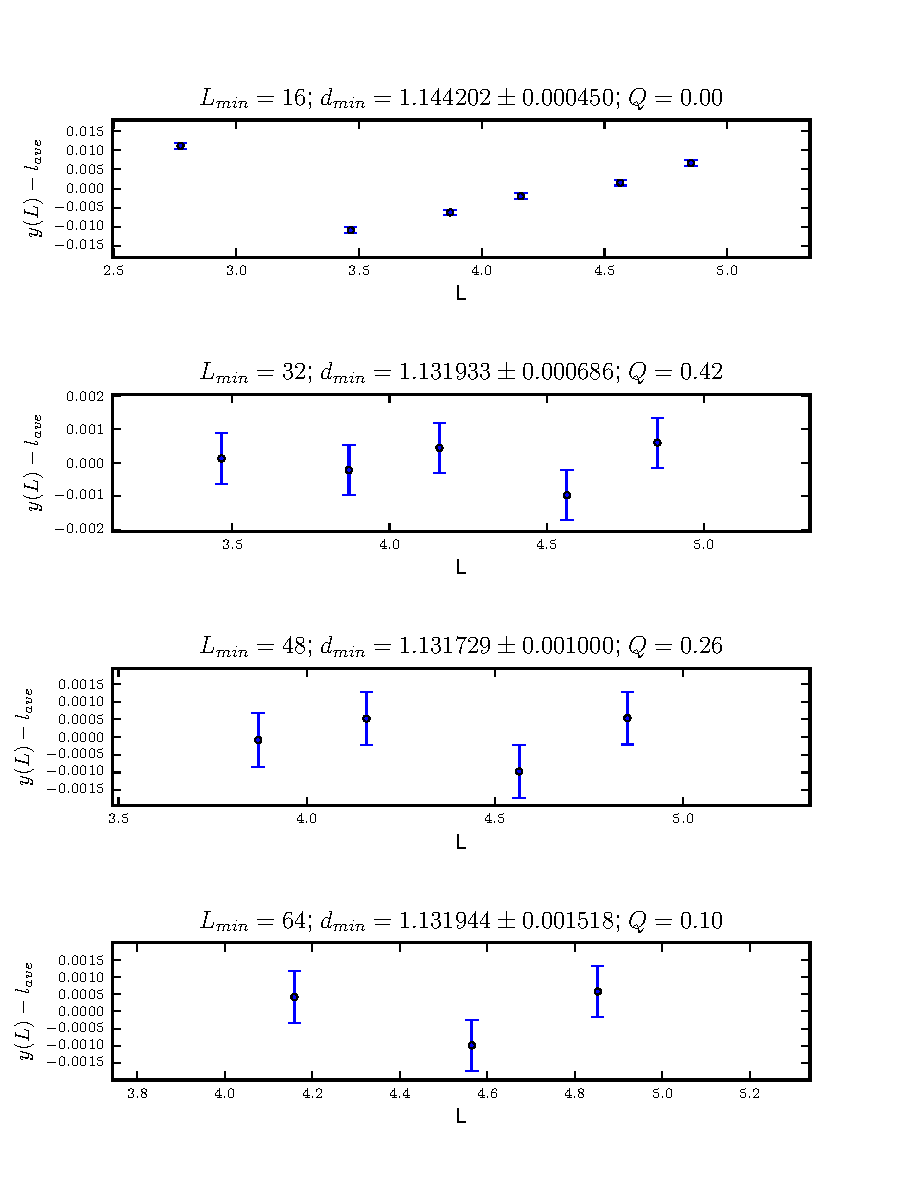
\includegraphics[width=.9\textwidth]{figures/d_min_D2q1_4601_fig_straightline}
\caption{$D=2, q=1, d_{min}$: linear fit of the ``log-log'' data (axes should be ``log'')}\label{fig:b}
\end{figure}

\begin{figure}[htp]
\centering
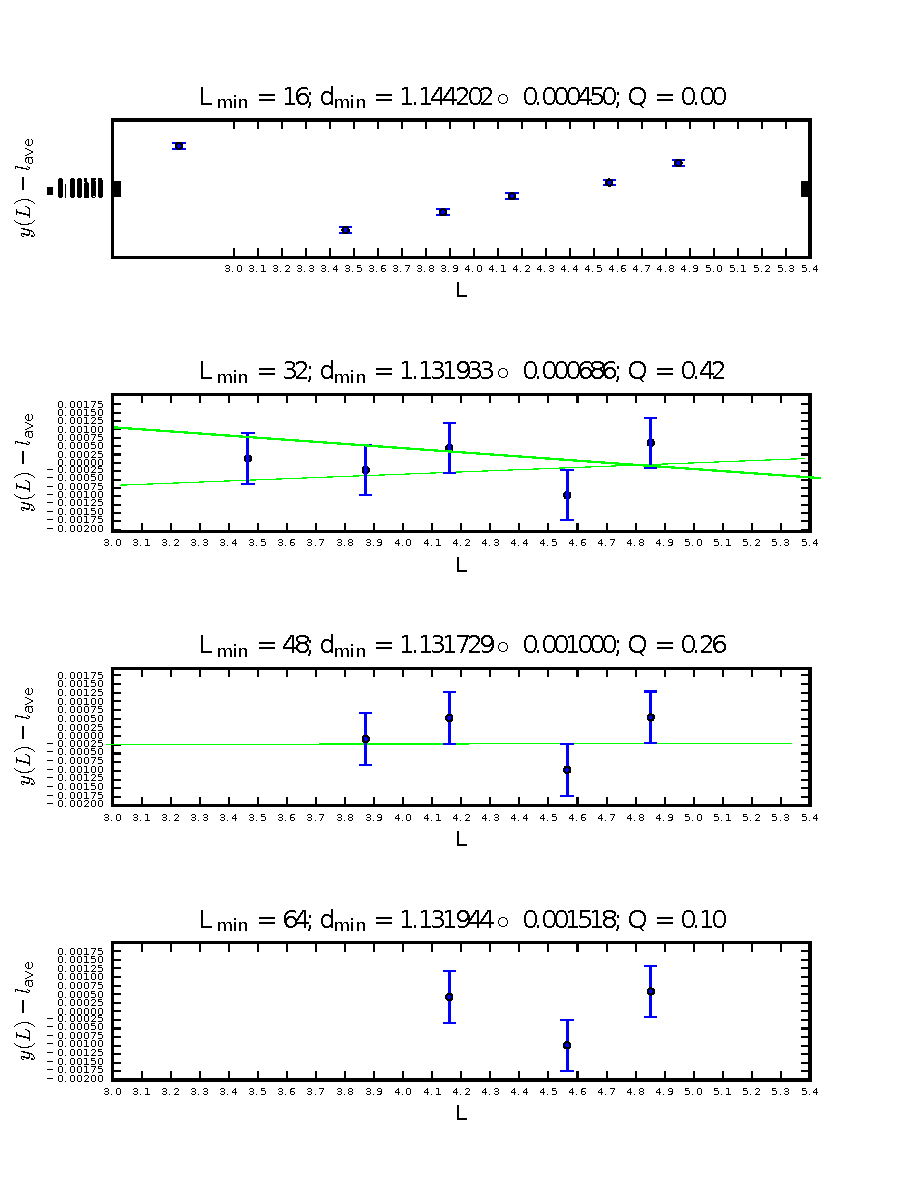
\includegraphics[width=.9\textwidth]{figures/d_min_D2q1_4601_fig_handfit_noboxes.pdf}
\caption{$D=2, q=1, L_{min}=32,d_{min}$: ``Hand-estimate'' of the error in the slope of the log-log data yields an error of $\pm 0.0010$ in the value for $d_{min}$ (axes should be ``log'').}\label{fig:b}
\end{figure}



\bibliography{/home/dwblair/dwbdocs/physics/bibfiles/dwbreferences}
\end{document}

